\section{Chapter 10: Interacting with Visualizations}
\graphicspath{ {pngs/ch10/} }

\secttoc

Cognitive systems designers wish to tighten the loop between human and
computer.
Mantra: ``overview first, zoom and filter, then details on demand.
Data manipulation loop: lowest level, select and move objects using eye-hand
coordination, delays are terrible. Exploration and navigation loop: analyst
finding way in a large visual data space. Faster navigation translates to
faster thinking.

Main focus is \textbf{epistemic actions:} activity intended to uncover new
information. Non-static displays.
Emphasis is placed on map-like layouts. May not be the optimal layout.
Another caveat: we wish to make interfaces transparent to the new user, but
expert users may be better off using the (possibly not-optimal) design they are
used to.

\begin{mdframed}\begin{multicols}{2}
\subsection{Data Selection Loop}
\begin{compactdesc}
\item[Choice reaction time] affected by distinctness of signals, amount of
    visual noise, stimulus-response compatibility. People react faster when
    allowed  to make mistakes. Hick-Hyman law, let $C$ is number of choices,
    $a$ and $b$ are empirically determined constants in
    \[
        \text{rxn. time} = a + b\log_2C
    \]
\item[2D positioning and scaling] Time to select a target of particular
    position and size described by Fitts' law. Describes an iterative
    eye-hand coordination process. Let $D$ be distance to the center of the
    target, $W$ be the width, and $b, a$  be empirically determined constants
    in
    \[
        \text{sel. time} = a + b\log_2 (D/W + 1.0)
    \]

\item[Hover queries]
    Extra information is revealed about an object when the mouse cursor
    passes over it. A delay is optional. Interactive query rate rise to several
    per second.
\item[Path tracing] continuous control. Let $v$ be the velocity of path
    tracing, $W$ be the path width and $\tau$ be a constant dependent on motor
    control system
    \[
        v = W\tau
    \]
\item[2 handed interaction] Guiard's (1987) Kinematic chain theory says the
    dominant performs detailed movements or manipulations, and the frame of
    reference is provided by the other hand.
\item[Learning] practice increases task performance, let $T_n$ be the
    time to complete the nth trial, $a$ represents steepness of learning
    curve:
    \[
        \log T_n = \log T_0 - a\log n
    \]
\item[Control compatibility] prior experience with a similar interface can
    increase learning speed
\end{compactdesc}
\end{multicols}\end{mdframed}




\begin{mdframed}\begin{multicols}{2}
\subsection{Exploration and Navigation Loop}
\begin{compactdesc}
\item[Locomotion and Viewpoint Control]
    Obstacles, margins, brinks, steps, slopes can be used as affordances to
    encourage and discourage visits. Smoothness is not necessary to detect
    motion, only identification of relative displacement is needed. Low FPS
    does cause other problems.
\item[Spatial navigation metaphors] good: apt, match the system, easy to
    understand. Navigation schemes can impose physical limits to the
    viewport, example: walking limits height seen.
    \begin{compactdesc}
    \item[World-in-hand] handle on a 3D environment is held and the whole world
        can be moved.
    \item[Eyeball-in-hand] user controls a camera. Most effective.
    \item[Walking] let users walk
    \item[Flying] relatively unconstrained 3D movement. Actual pilots have
        difficulty: unnecessary banking while turning, won't stop or go
        backwards
    \end{compactdesc}
\item[Wayfinding, Cognitive maps] first: landmarks are learned, 2nd: routes are
    learned, last: cognitive spatial map. Experiment: brief exposure to a map
    was equivalent to about a year of working in a large building. Overviews
    should be provided for large spaces.
\item[Terrain features] may not be mentally encoded as 3D objects, but as
    viewpoint-dependent mental images.
\item[Landmarks, Borders, Place] in the hippocampus: border cells signal
    impenetrable barriers, place cells signal specific locations, and grid cells
    contain updated map of where we are, relative to surroundings.
    Interesting: subjects provided with 3D overviews of a city's landmarks
    navigated better than those given pictures or verbal descriptions.
\end{compactdesc}
\end{multicols}\end{mdframed}





\begin{mdframed}\begin{multicols}{2}
\begin{compactdesc}
\item[Frames of Reference] a map is one of many exocentric views.
\item[Egocentric Frame of Reference] our subjective view of the world. Anchored
    to the head or torso, not direction of gaze. We are accustomed only to pan
    or tilt, not roll.
\item[Exocentric Frames of Reference]  God's-eye and wingman's are called
    tethered because they follow a moving object.
    \begin{compactdesc}
    \item[Another person's view] someone else's egocentric view
    \item[Over the shoulder view] behind and to the side of the head of an
        individual
    \item[God's-eye view] from above and behind. Common in video games
    \item[Wingman's view] from the side.
    \end{compactdesc}
\item[Map orientation]
    Track-up preferable, but experienced navigators or distant collaborators
    prefer north-up.
    \begin{compactdesc}
    \item[North-up view] Orthographic. Classical map view. Vehicle in the middle.
    \item[Track-up view] Orthographic. Heading of the vehicle is the vertical up
        direction.
    \item[Track-up perspective view] God's-eye view above and behind the
        vehicle.
    \end{compactdesc}
\end{compactdesc}
\begin{figure}[H] \centering
    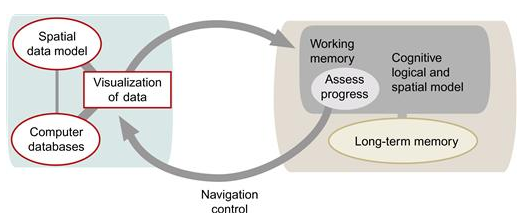
\includegraphics[width=\linewidth]{navigation_loop.png}
    \caption{The navigation loop}
\end{figure}
\end{multicols}\end{mdframed}





\begin{mdframed}\begin{multicols}{2}
\subsection{Focus, Context, Scale in Nonmetaphoric Interfaces}
\begin{compactdesc}
\item[Focus-context problems]
    Focus is the pattern, which need not be small, context is the larger data
    landscape.
    \begin{compactdesc}
    \item[Spatial scale] Information based on real-world scales
    \item[Structural scale] software example: a single line of code, a
        subroutine, at the object level, at the system level. Many levels
        of detail
    \item[Temporal scale] understanding the timing of events at several
        scales.
    \end{compactdesc}
\item[Distortion techniques] Hyperbolic tree browser. The fish-eye lens.
    Some layouts allow multiple foci.
    Such techniques may render details along the border between focus and
    context unreadable.
\item[Rapid Zooming Techniques] Quick transitions. Ideal rate of zoom is 3 to 4
    scale units per second. People vary from 2 to 8.
\item[Key issue] how fast can views be changed? Is it smooth enough to maintain
    identity of objects? Landmarks consistent?
\item[Elision Techniques] parts of a structure are hidden until needed.
\item[Multiple Simultaneous Views] large data space? One window shows an
    overview, and others show expanded details. Link the windows w/ Gestalt
    principles.
\end{compactdesc}
\begin{figure}[H] \centering
    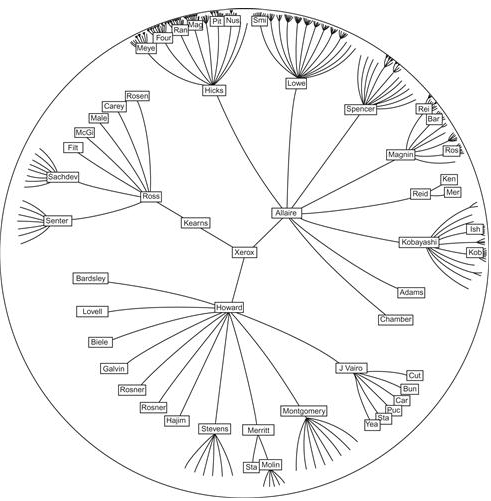
\includegraphics[width=0.6\linewidth]{hyperbolic_tree.png}
    \caption{A hyperbolic tree. Far away nodes are clicked to focus on them.}
\end{figure}
\end{multicols}\end{mdframed}



